\section{Introducción}
En esta práctica crearemos un chat multiusuario usando el paradigma cliente-servidor.
El servidor será un proceso alojado en alguno de los ordenadores de la comunicación.
El servidor será el encargado de mandar el mensaje a los usuarios implicados en la comunicación, y solamente a ellos.
La práctica será realizada en \textit{JAVA}.

La estructura del programa es la siguiente.

\begin{figure}[h]
	\centering
	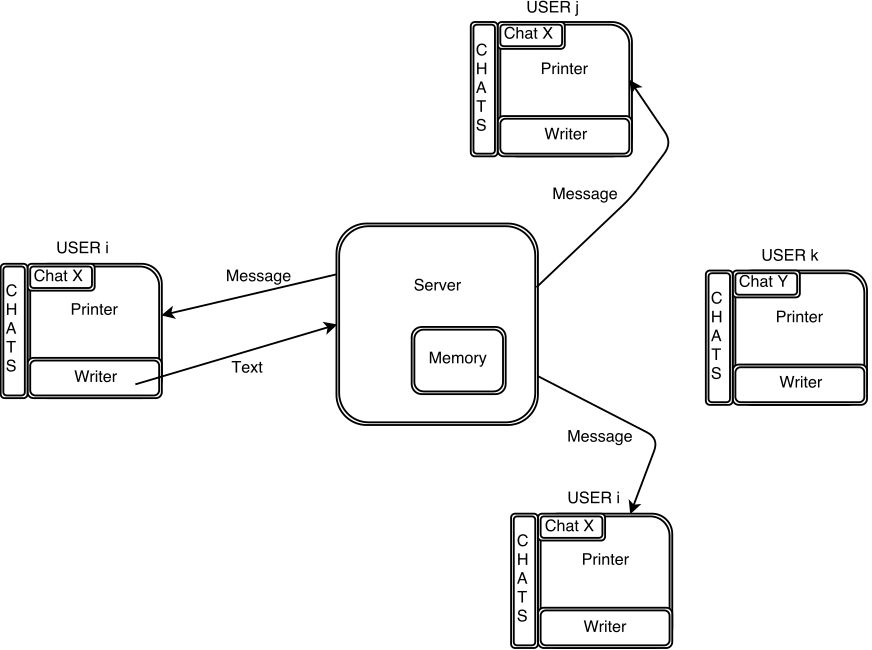
\includegraphics[width=0.9\textwidth]{./Imagenes/chat.png}
\end{figure}